

\chapter{Data Types}
\label{chap:data_types}

\section{Introduction}

Choosing the right data types plays an important role in writing an otpmized code and deploy it to target. This chapter explains the data type options in \verb|HLS| and their related optimisation and development techniques.

\todo{data types intro} \uti{data types intro:}

\begin{itemize}

\item \textit{To adjust the introduction later}

\item \textit{This chapter needs I think a review about data types in C and C++}

	\begin{itemize}
	\item \textit{To see if there exist some differences between the 2 languages}
	
	\item \textit{To make link if possible between data types in a PC, MCU and FPGA}
	\end{itemize}

\end{itemize}

\newpage
\section{Native Data Types}

Programming languages such as \verb|C| and \verb|C++| support some native or builtin data types (\verb|char|,\verb|int|,$\cdots$), which can be modified using \textit{modifiers}, such as \verb|signed|,\verb|short|,$\cdots$

\begin{figure}[h]
\centering
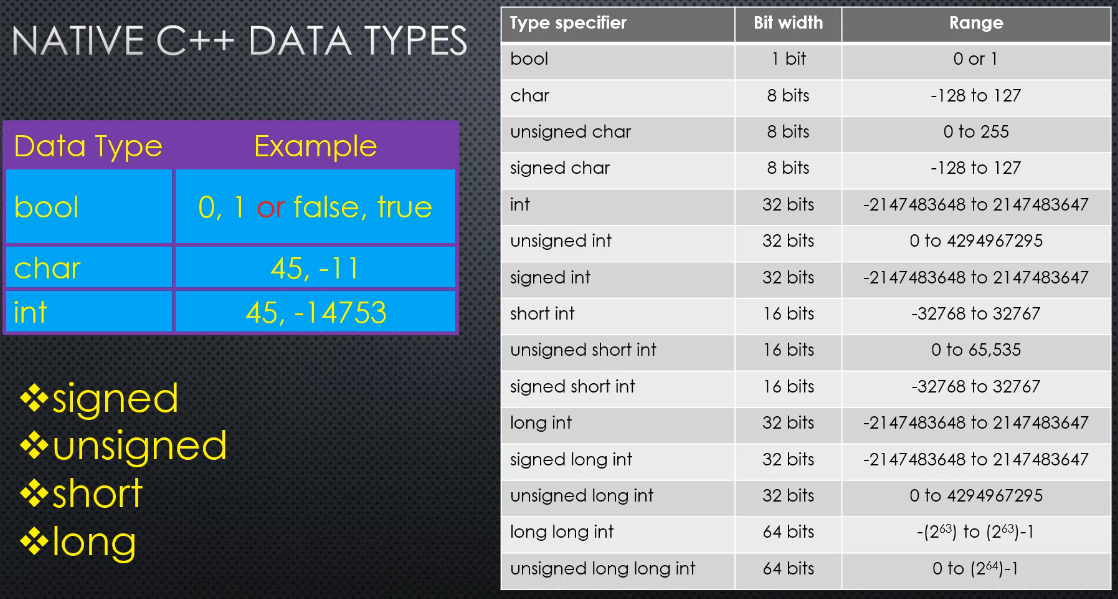
\includegraphics[scale=0.35,frame]{Figures/data_types/data_types_modifiers}
\caption{Data types, modifiers and ranges}
\label{fig:data_types:data_types_modifiers}
\end{figure}

\newpage
\section{Synthesis and Hardware Consideration}

Given some data type, the variables in our code will be mapped to hardware. During this mapping process, some optimization can be made such as eliminating some variables or creating some new intermediate ones.\\ 

Examples are shown in \autoref{fig:data_types:function_example}.

\begin{figure}[h]
\centering
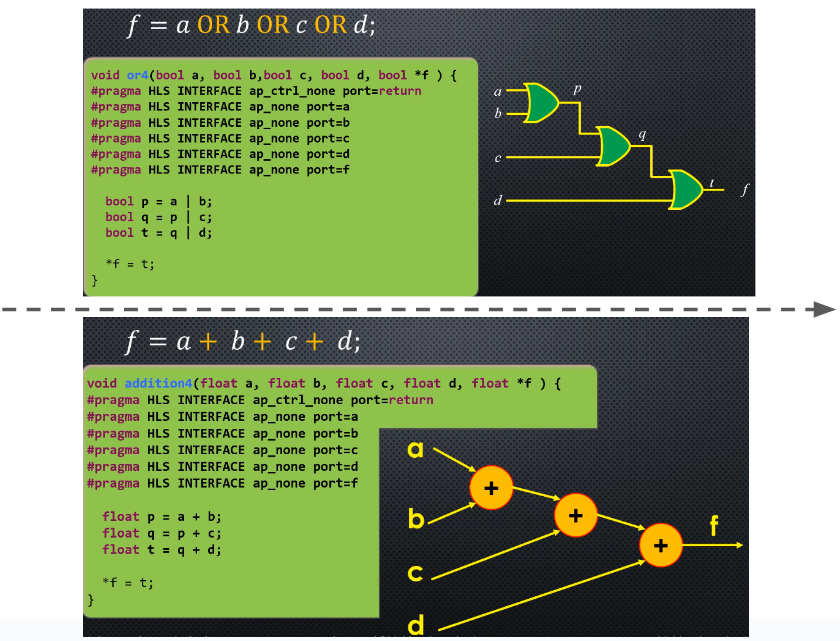
\includegraphics[scale=0.45,frame]{Figures/data_types/function_example}
\caption{Some function example: boolean and arithmetic}
\label{fig:data_types:function_example}
\end{figure}

For the $\mathrm{1}^\mathrm{st}$ system (the boolean function), the circuit can be optimized using the assocaitivity property of \verb|OR| gate, and this result having a system of $t_p \, = \, 3 \delta$ to $t_p \, = \, 2 \delta$ as shown in \autoref{fig:data_types:optim_example}. As for the $\mathrm{2}^\mathrm{nd}$ function (the arithmetic function), the \verb|+| operator will be mapped to adder circuits.

\newpage
\begin{figure}[h]
\centering
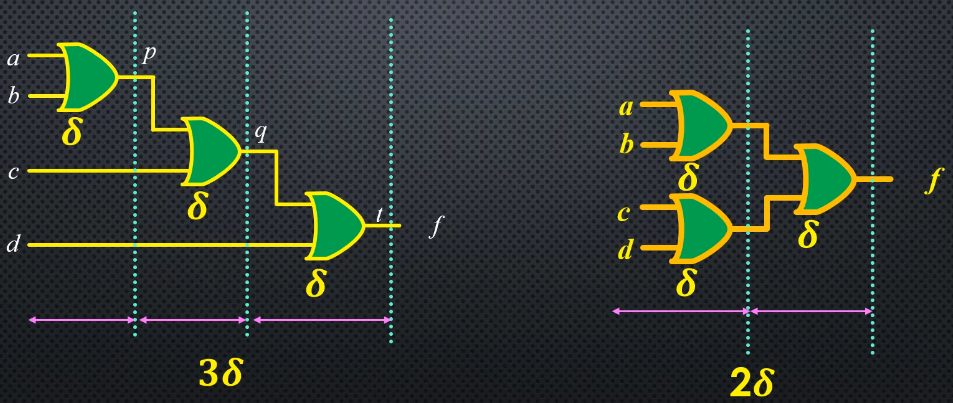
\includegraphics[scale=0.35,frame]{Figures/data_types/optim_example}
\caption{Optimzation of $t_p$}
\label{fig:data_types:optim_example}
\end{figure}


\newpage
\section{Bit Precision}
 
In FPGA programming, it is common to use \textit{arbitrary bit width} with signals, buses,$\cdots$ to have an optimzed solution.
Native \verb|C| data types comes usually with a multiple of 8 (1,8,16,32,$\cdots$), and if we want to implement some circuit let's say a 19 bit multiplier, we can use 32 bit but it's not efficient. That's why the motiviation behind arbitray bit width need.\\

In \verb|HLS|, there exist 2 libraries: 1 for \verb|C| and 1 for \verb|C++|. In this course we focus the one in \verb|C++|. An example is shown in \autoref{fig:data_types:bitwidth_cpp}.

\begin{figure}[h]
\centering
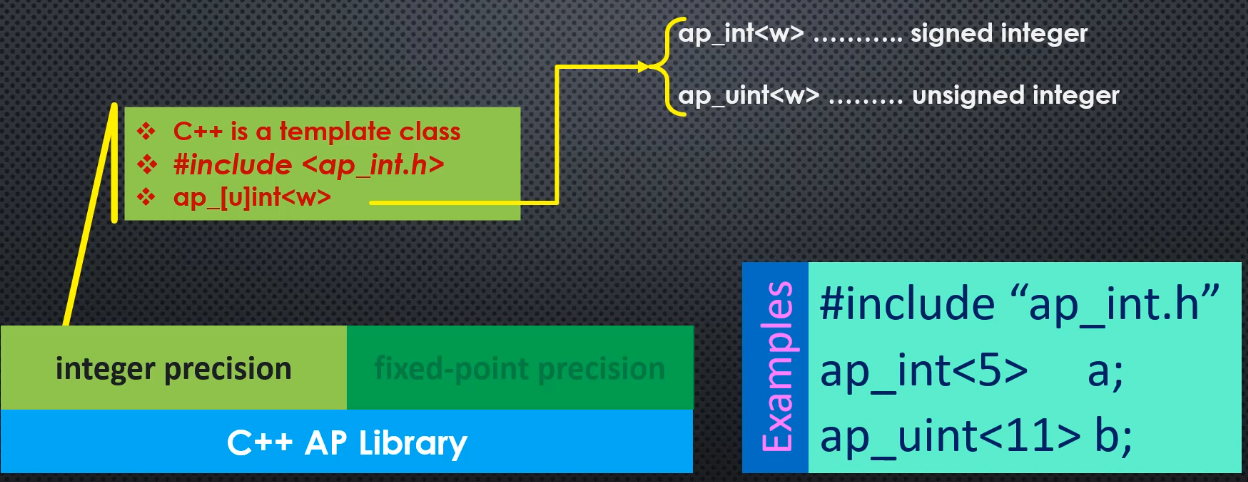
\includegraphics[scale=0.35,frame]{Figures/data_types/bitwidth_cpp}
\caption{Example of C++ library for arbitrary bit width support}
\label{fig:data_types:bitwidth_cpp}
\end{figure}

\todo{Arbitrary width bit in C} \uti{Arbitrary width bit in C:}

\begin{itemize}

\item \textit{To see later the C library, some search about it and some documentation}

\end{itemize}

\newpage
\section{Initialization}

Initialization and assignment is done via class constructor and operator overloading. An example is shown in \autoref{fig:data_types:init_bitwidth_ex}

\begin{figure}[h]
\centering
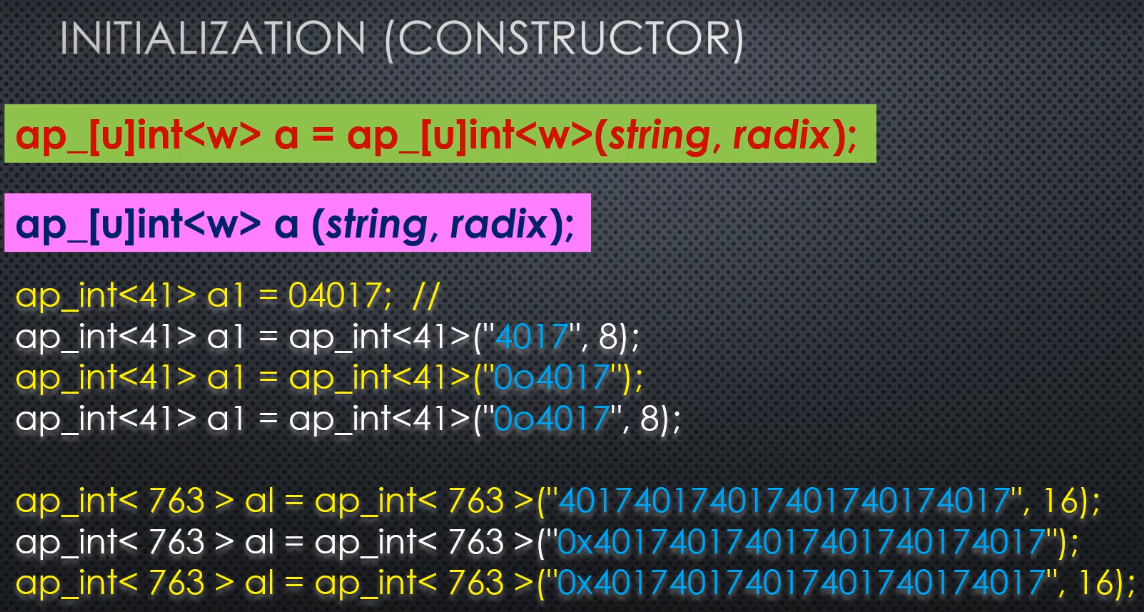
\includegraphics[scale=0.35,frame]{Figures/data_types/init_bitwidth_ex}
\caption{Initialization Example}
\label{fig:data_types:init_bitwidth_ex}
\end{figure}

\begin{itemize}

\item the \verb|ap_int<>| takes 2 argument: a string reprensenting the value and radix (the base), which can be 2,8,10 or 16

	\begin{itemize}
	\item If the $\mathrm{2}^\mathrm{nd}$ argument (the radix) is not provided, the constructor \textit{can infer the base} from the string argument, using prefix \verb|0b| (binary),\verb|0o|(octal), and \verb|0x|(hexadecimal)
	\end{itemize}

\item In $\mathrm{1}^\mathrm{st}$  example in \autoref{fig:data_types:init_bitwidth_ex}, we have 4 different ways of initializing a variable \verb|a1| of width 41 bits with an octal value

	\begin{itemize}
	\item In \verb|C++|, when we intialize a number and put \verb|0| in front, the number is treated as octal (the $\mathrm{1}^\mathrm{st}$ way)
	\end{itemize}

\item In the $\mathrm{2}^\mathrm{nd}$ example in \autoref{fig:data_types:init_bitwidth_ex}, we have 3 ways of initializing variable \verb|al| of width 763 bits with hexadecimal number

\end{itemize}

\newpage
\autoref{fig:data_types:format_printing} presents the ways of printing in the correct base, using \verb|std::oct|,$\cdots$

\begin{figure}[h]
\centering
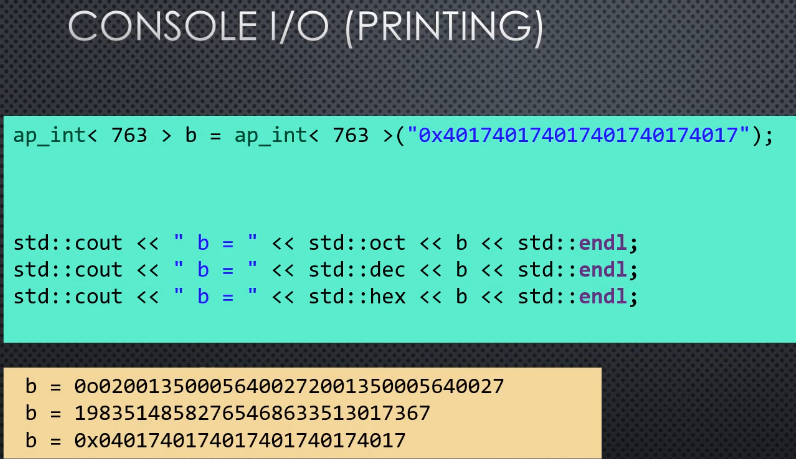
\includegraphics[scale=0.35,frame]{Figures/data_types/format_printing}
\caption{Initialization Example}
\label{fig:data_types:format_printing}
\end{figure}


\newpage
\section{Bit Precision: Assignment}

\autoref{fig:data_types:var_assignment} shows an example of assignment in \verb|HLS| using the \verb|ap_int.h| also.

\begin{figure}[h]
\centering
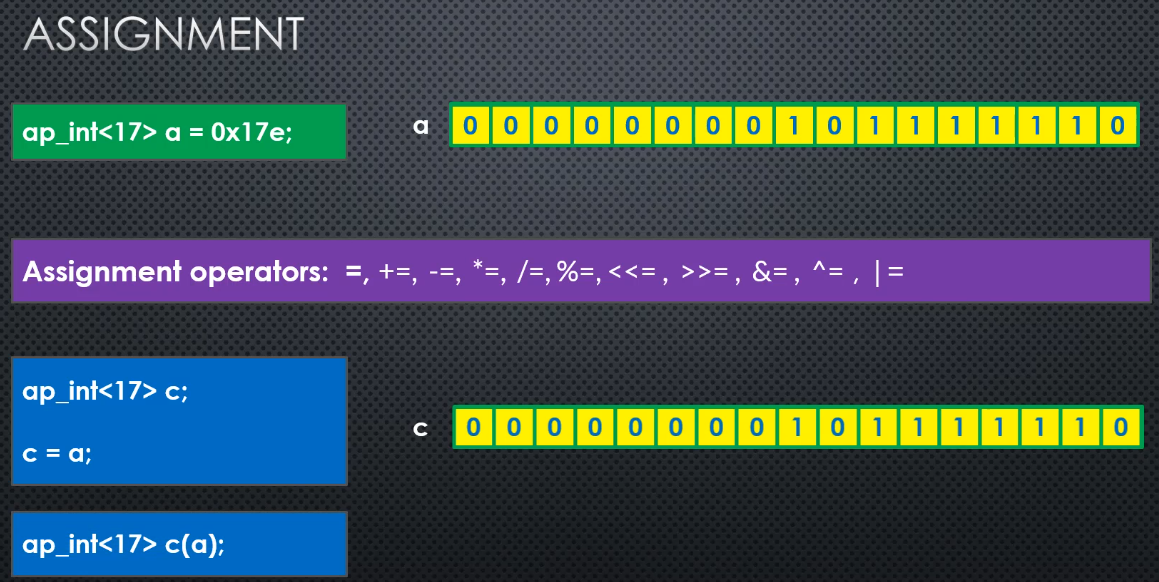
\includegraphics[scale=0.35,frame]{Figures/data_types/var_assignment}
\caption{Assignmnet in HLS}
\label{fig:data_types:var_assignment}
\end{figure}

\begin{itemize}

\item Notice that, a variable can also be assigned to another variable upon its declaration, thanks to the constructors provided by arbitrary precision class template

\end{itemize}

\todo{C++ features and template} \uti{C++ features and template:}

\begin{itemize}

\item \textit{To make a review about C++ programming later , the concept of template, constructor,$\cdots$}

\item \textit{There are many concepts related to constructor and initialization in OOP that I skipped for now in this course}

\item \textit{When I finish my C++ course, I will get back to it later}

\end{itemize}


\newpage
\subsection{Wider and Narrower Assignment}

What happen if we assign some variables having a \textit{different bit width} ? We explore this situation in this section. An example is shown in \autoref{fig:data_types:assignment_types}.


\begin{figure}[h]
\centering
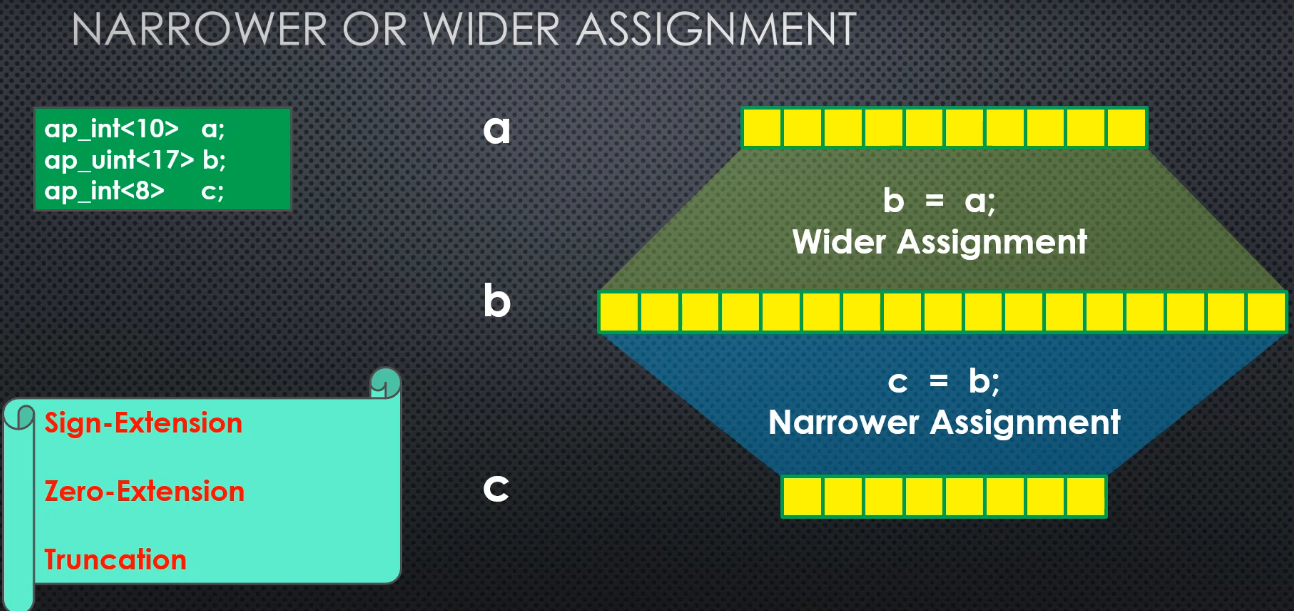
\includegraphics[scale=0.35,frame]{Figures/data_types/assignment_types}
\caption{Assignmnet types: wide and narrow}
\label{fig:data_types:assignment_types}
\end{figure}

\begin{itemize}

\item We have 3 variables: \verb|a|,\verb|b| and \verb|c|

\item \verb|b = a|: we assign \verb|b| to \verb|a|, so the question we need to answer

	\begin{itemize}
	\item this is a \textit{wide assignment} $\leftrightarrow$ what should we do with the extra bits in \verb|b|?
	\end{itemize}

\item \verb|c = b|: we assign \verb|b| to \verb|c|

	\begin{itemize}
	\item This is a \textit{narrow assignment} $\leftrightarrow$ what should we do with missing bits in \verb|b| variable ?
	\end{itemize}

\item The answer to these questions depends on the \textit{signdness}, and we have 3 techniques: sign extension, zero extension, and truncation

\end{itemize}

Let's see how these techniques work.\\

\newpage
\subsection{Sign Extension}

Sign extension is applied when we move from (assing) narrow signed to wider variable.

The value is sign extended to the width of the destination variable, regardless of its its signedness. An example is shown in \autoref{fig:data_types:sign_extension}.


\begin{figure}[h]
\centering
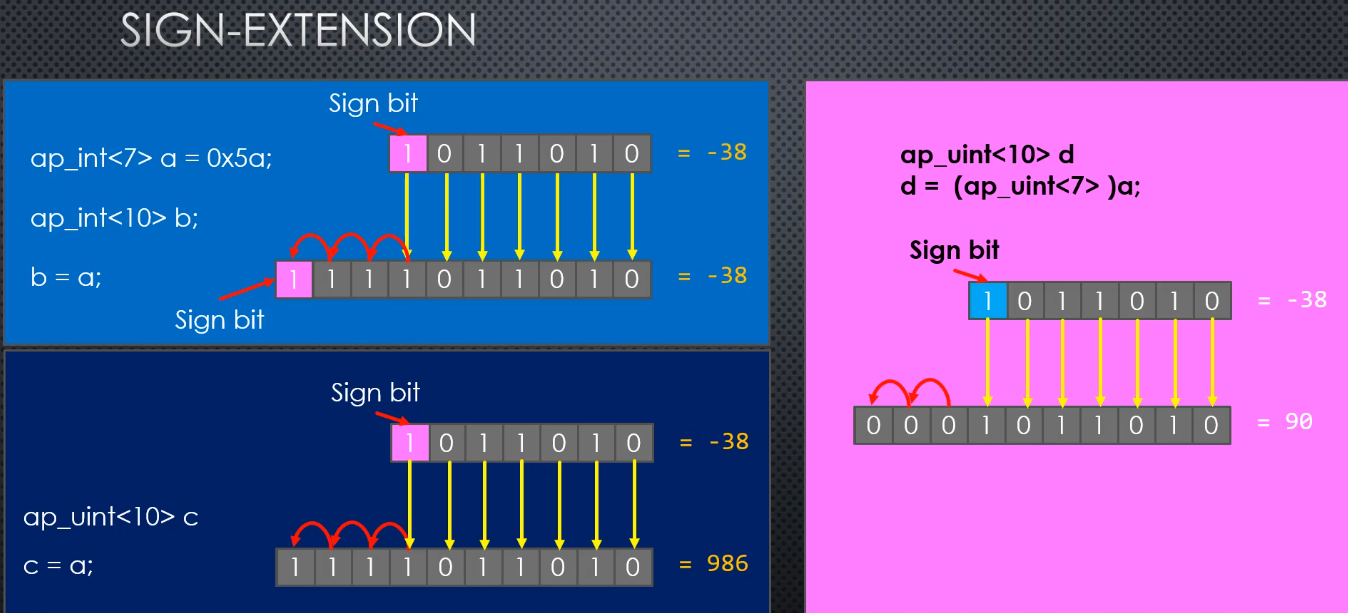
\includegraphics[scale=0.35,frame]{Figures/data_types/sign_extension}
\caption{Sign Extension Example}
\label{fig:data_types:sign_extension}
\end{figure}

\begin{itemize}

\item 2 cases are shown in \autoref{fig:data_types:sign_extension}: \verb|b = a| and \verb|c = a|

	\begin{itemize}
	\item The difference is the type of variable \verb|c| is unsigned integer (\verb|ap_uint()|)
	\end{itemize}

\item In the $\mathrm{1}^\mathrm{st}$ case \verb|b = a|: we fill the extra bits of \verb|b| with the same sign bit of \verb|a|.

\verb|b| holds the same value of \verb|a|

\item In the $\mathrm{2}^\mathrm{nd}$ case \verb|c = a|: also sign bit extension is applied to \verb|c| even though \verb|c| is unisgned integer, and thus \verb|c| will not hold the same value of \verb|a|

\item The $\mathrm{3}^\mathrm{rd}$ example uses the concept of \textit{type casting}: since \verb|a| is a signed integer, we can type caste it to unisgned integer and then assign it to variable \verb|d|

	\begin{itemize}
	\item In this case, signed extension won't happen, and \verb|d| is filled with 0
	\end{itemize}

\end{itemize}

\todo{number representation} \uti{number representation:}

\begin{itemize}

\item \textit{To review number representation and base conversion, because I don't know why c doesn't hold the same value of b or a}	

\end{itemize}

\newpage
\subsection{Zero Extension} 
 
For zero extension, that is filling extra bits with 0, the source variable need to be unsigned. Examples are shown in \autoref{fig:data_types:zero_extension}. 


\begin{figure}[h]
\centering
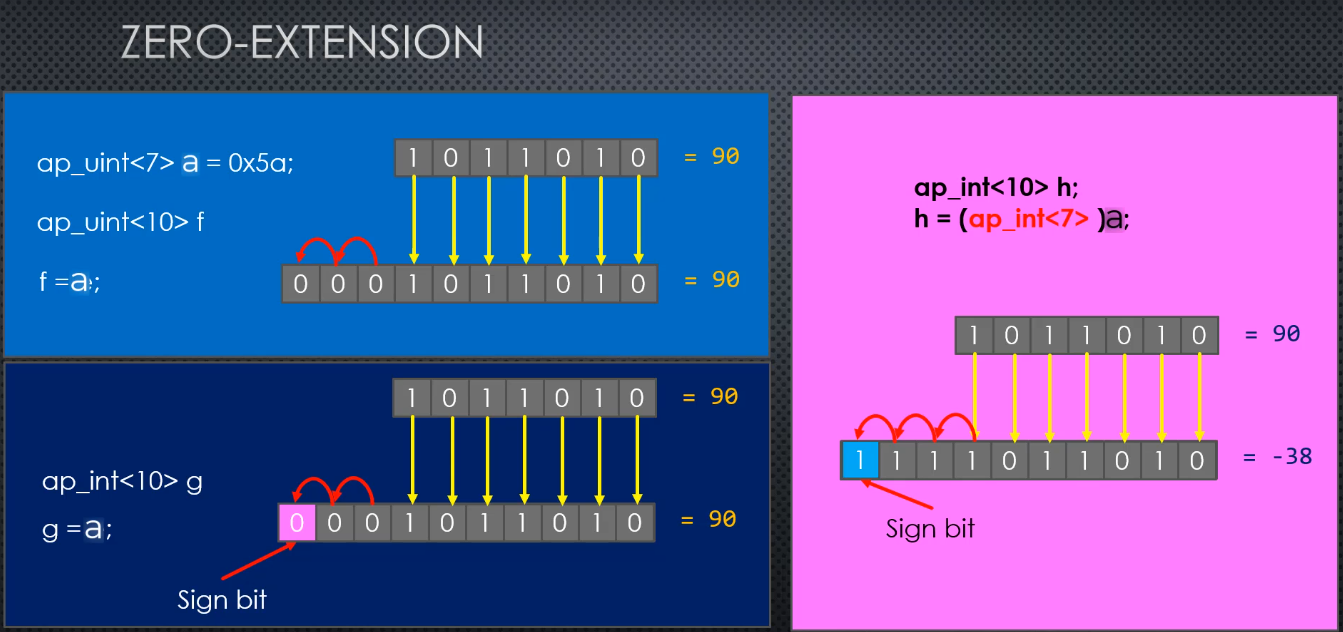
\includegraphics[scale=0.35,frame]{Figures/data_types/zero_extension}
\caption{Zero Extension Example}
\label{fig:data_types:zero_extension}
\end{figure}

\begin{itemize}

\item We have a source variable \verb|a| which is unsigned

\item we have 2 operation: 

	\begin{itemize}
	\item \verb|f = a|, \verb|f| is also unisgned
	
	\item \verb|g = a|. \verb|g| is signed
	\end{itemize}

\item In the $\mathrm{3}^\mathrm{rd}$ operation  where we have variable \verb|h| and type casting is used, the value \verb|a| is changed during assignment from 90 to -38

\end{itemize}

\newpage
\subsection{Truncation}

Now we take the $\mathrm{2}\mathrm{nd}$ case, that is moving from wider to narrow variable, which is known as truncation.

\begin{figure}[h]
\centering
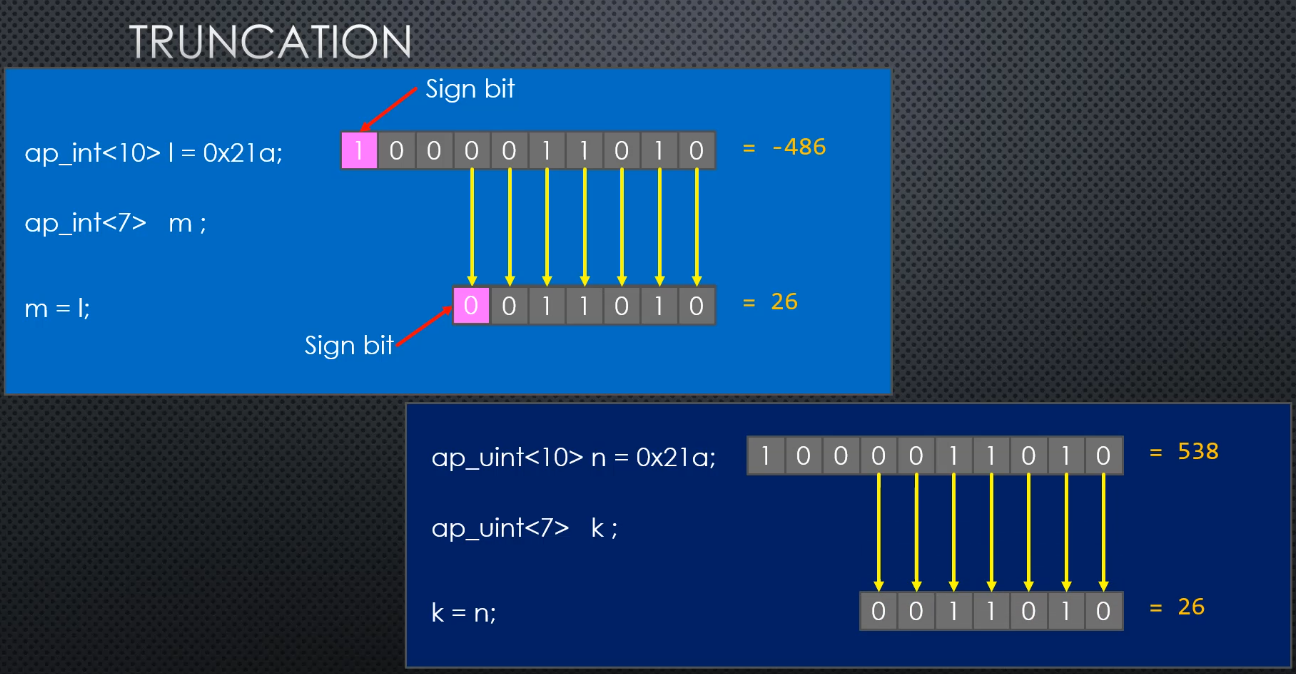
\includegraphics[scale=0.35,frame]{Figures/data_types/truncation}
\caption{Truncation Example}
\label{fig:data_types:truncation}
\end{figure}

\begin{itemize}

\item In truncation, MSB is lost, and no special treatment for signed bit, which may lead to unexpected behavior

\end{itemize}

\newpage
\section{Bit Level Operation} 

Now we introduce several bit level operation. 


\subsection{Concatenation}

\begin{figure}[h]
\centering
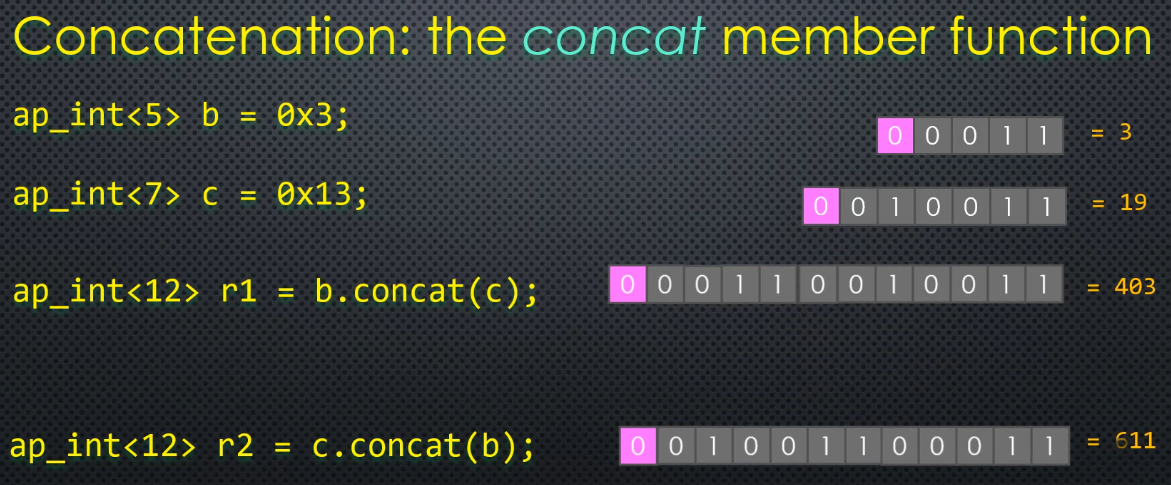
\includegraphics[scale=0.35,frame]{Figures/data_types/concat}
\caption{Concatenation}
\label{fig:data_types:concat}
\end{figure} 
 
\begin{itemize}

\item \verb|b.concat(c)|: \verb|b| will be in the upper part, and \verb|c| is in the lower part

\end{itemize} 
 
Concatenation can also be done using the comma overloaded operator as shown in \autoref{fig:data_types:concat_comma}.
 
\begin{figure}[h]
\centering
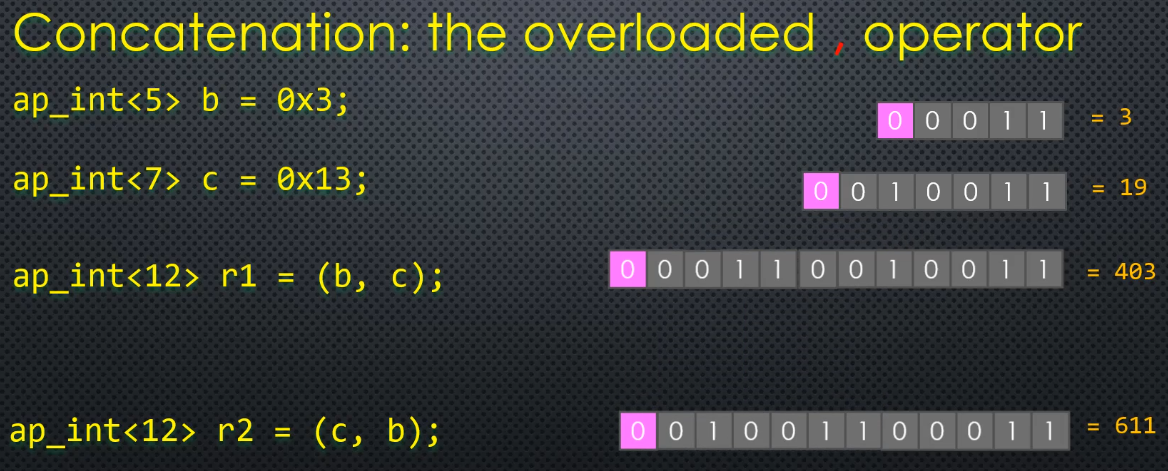
\includegraphics[scale=0.35,frame]{Figures/data_types/concat_comma}
\caption{Concatenation}
\label{fig:data_types:concat_comma}
\end{figure}  
 
\newpage  
\subsection{Bit Selection} 
 
Bit selection can be done using the overlaoded \verb|[]| operator as shown in \autoref{fig:data_types:bit_selection}.

\begin{figure}[h]
\centering
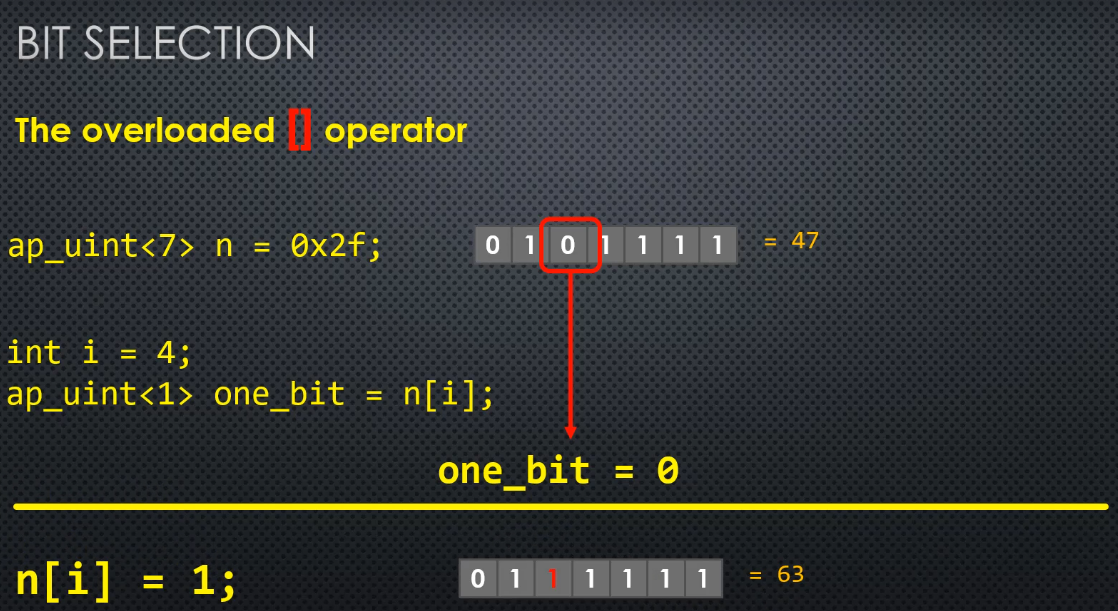
\includegraphics[scale=0.35,frame]{Figures/data_types/bit_selection}
\caption{Bit Selection}
\label{fig:data_types:bit_selection}
\end{figure} 
 
\newpage 
\subsection{Range Selection} 
 
Selecting a range of consecutive bits can be done the \verb|range()| function as shown in \autoref{fig:data_types:range_bits}.

\begin{figure}[h]
\centering
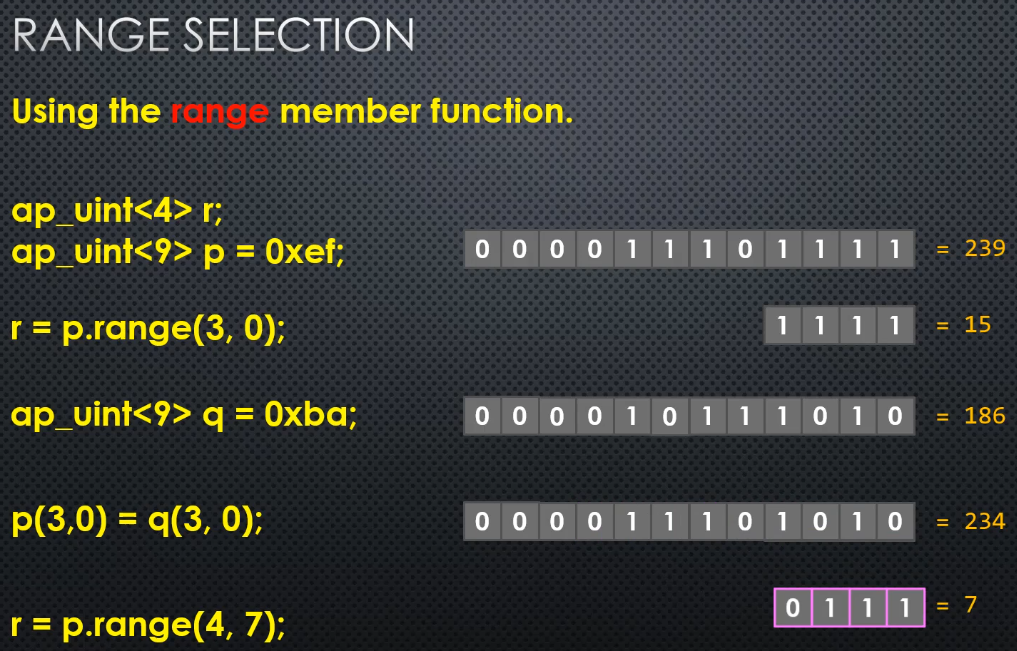
\includegraphics[scale=0.35,frame]{Figures/data_types/range_bits}
\caption{Selecing a range of bits}
\label{fig:data_types:range_bits}
\end{figure}
 
 
 \uti{Range bits:} \todo{Range bits}

\begin{itemize}

\item \textit{There are some mistake int the $\mathrm{2}^\mathrm{nd}$ example of \autoref{fig:data_types:range_bits}}

\item \textit{I will search an example for the correct use of arguments}

\end{itemize}

\newpage
\subsection{Bitwise Logical Operator}

We continue exploring bitwise operations with logical operator on a bitlevel as shown in \autoref{fig:data_types:bitwise_operations}.

\begin{figure}[h]
\centering
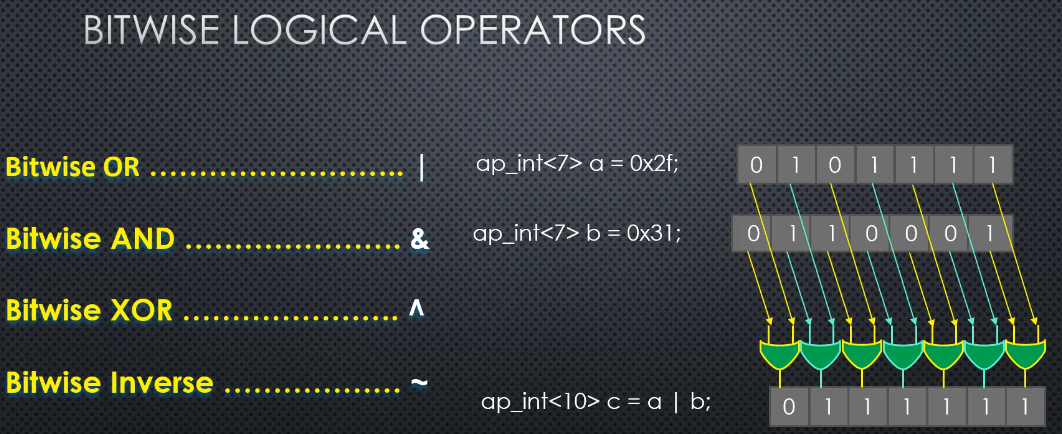
\includegraphics[scale=0.35,frame]{Figures/data_types/bitwise_operations}
\caption{Bitwise Operation Example}
\label{fig:data_types:bitwise_operations}
\end{figure}

\begin{itemize}

\item Bitwise logical operators all return a value with a width
that is the maximum of the widths of the two operands

\item They are treated as unsigned if and only if both operands are unsigned

\item Otherwise, it is of a signed type, sign-extension (or zero-padding) may occur, based on the signedness of the expression, not the destination variable

\end{itemize}

\uti{Bitwise logical operator:} \todo{Bitwise logical operator}

\begin{itemize}

\item \textit{To make sure of this concepts of max width return, and zero extension, because in emebdedded C I don't think I encountered such concepts before}

\end{itemize}

\newpage
\subsection{Reduced Logical Function}

Reduced functions apply a given operator to all bits of an arbitrary precision value and return a one-bit result. An example is shown in \autoref{fig:data_types:reduced_logical_function}.

\begin{figure}[h]
\centering
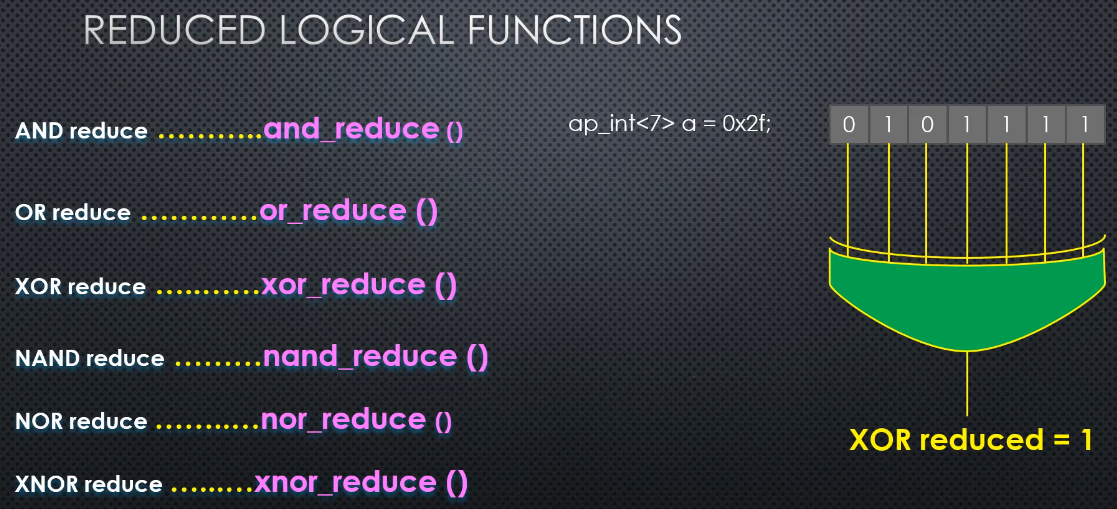
\includegraphics[scale=0.35,frame]{Figures/data_types/reduced_logical_function}
\caption{Reduced Logical Function}
\label{fig:data_types:reduced_logical_function}
\end{figure}

\uti{Reduced Logical Function:} 

\todo{Reduced Logical Function}

\begin{itemize}

\item \textit{There are no mentions for the rules of such operation, to be seen later}

\end{itemize}

\newpage
\subsection{Test,Set Clear}

Set,reset and test function example are shown in \autoref{fig:data_types:set_reset_test}.

\begin{figure}[h]
\centering
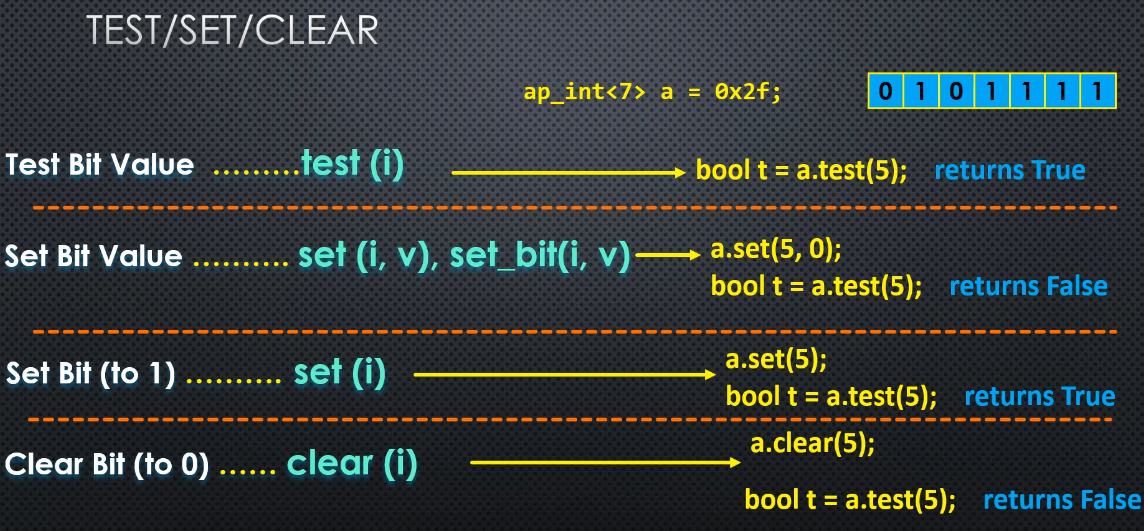
\includegraphics[scale=0.35,frame]{Figures/data_types/set_reset_test}
\caption{Test,Set and Clear}
\label{fig:data_types:set_reset_test}
\end{figure}


\newpage
\subsection{Bit Shift and Rotate}

Now we move to bit shifting operations. Shift operation are performed right and left direction as shown in \autoref{fig:data_types:bit_shift}.

\begin{figure}[h]
\centering
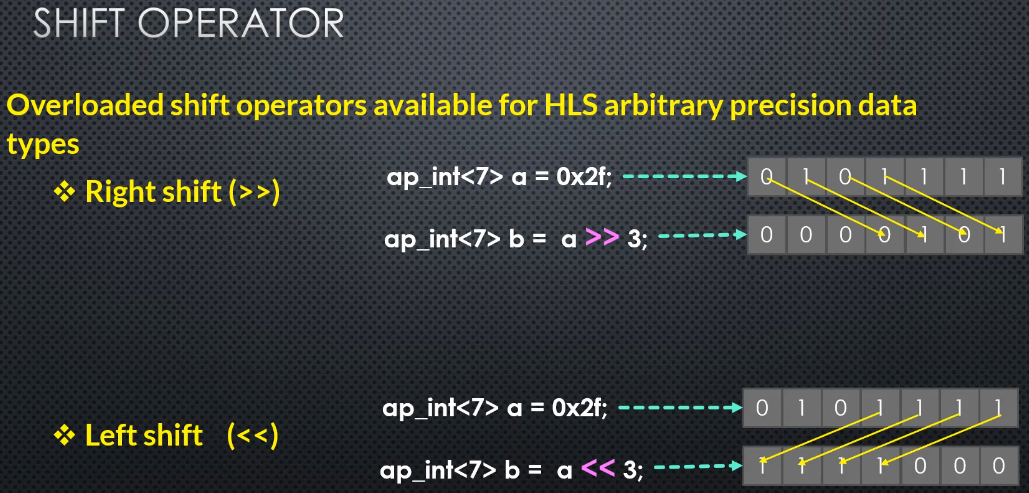
\includegraphics[scale=0.35,frame]{Figures/data_types/bit_shift}
\caption{Bit shift operation}
\label{fig:data_types:bit_shift}
\end{figure}

Also in \verb|HLS| we have some functions to do some rotation to the bits, also in left and right as shown in \autoref{fig:data_types:bit_rotate}.

\begin{figure}[h]
\centering
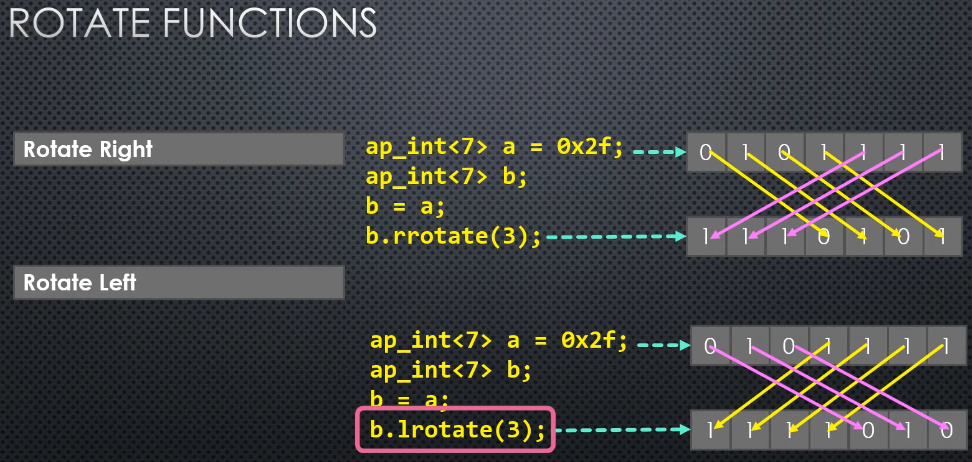
\includegraphics[scale=0.35,frame]{Figures/data_types/bit_rotate}
\caption{Bit rotation}
\label{fig:data_types:bit_rotate}
\end{figure}





